\noindent
Side-channel attacks leak information between protection domains outside of the normal information flow of a system.
In late 2017 a new class of side-channel attacks was discovered impacting CPUs from all major vendors~\cite{lipp:meltdown, kocher:spectre}.
These attacks---termed transient execution attacks---exploit details of how modern processors use speculative execution to run more quickly. 

Transient execution attacks represent a concern for system developers because providing isolation is a key security responsibility for many kinds of software.
For instance, an operating system must not allow processes running on the same machine to inadvertently leak information between one another, and web browsers must ensure that JavaScript running on one website cannot access state belonging to other sites.
System developers have deployed a range of techniques devised to mitigate the impact of these transient execution attacks, but unfortunately they can introduce significant performance costs.

The overhead caused by mitigations is present on vulnerable processors dating from before the discovery of the attacks and also at least to some degree on all major commercial CPUs released after their discovery.
This thesis (i) measures how overhead has evolved over subsequent generations of processors, and (ii) since processors from 2017 and earlier will remain in use for years to come, presents a new operating system design to reduce OS level overheads those CPUs.

% Many hundreds of millions of vulnerable computer processors are currently in use, so simply replacing them all isn’t by itself a viable solution.
% Worse still, computer architectural approaches to solve transient execution attacks remains an open area of research, except on the simplest of processors.

% Nonetheless, generations of processors designed after the discovery of transient execution attacks have improvements that make them inherently less susceptible to attack.
% It is desirable to understand how this was achieved yet little has been published on exactly what changes were made.
% The focus of this thesis is on understanding and reducing the impact of mitigations on performance.

\section{Transient Execution Attacks}
Speculative execution is an optimization used in the design of modern processors to drastically improve their performance, by enabling them to do useful work during times when they would otherwise be stalled waiting to load information from memory.
When the CPU reaches a conditional branch instruction that it doesn't yet know whether will be taken or not, it predicts the outcome and then starts executing instructions that would follow.
The prediction is based on prior executions of that same instructions and any other heuristics the processor may have.

Usually the branch prediction is correct and the speculatively executed instructions can be committed.
When the prediction is incorrect, the CPU rolls back the architecturally visible results of the instructions executed after the branch.
However, in general when reverting transiently executed instructions, their microarchitural effects---like inserting or evicting lines from the cache---are not undone.
Observing the  microarchitural effects of speculatively executed instructions enables transient execution attacks.

\subsection{Example Attack}
\begin{figure}[h]
\begin{lstlisting}[language=C, style=codeStyle]
if (index < array_size) {
    int v = array2[array1[index] * 256];
    ...
}
\end{lstlisting}
\caption{Example code for a Spectre V1 attack}
\label{fig:spectre-code}
\end{figure}
Spectre V1 was one of the earliest attacks discovered and leaks information between different processes, between a process and the operating system kernel, or between a sandbox and the code running within.
The attack relies on a specific sequence of instructions called a ``gadget'' to be located in the victim's code region (e.g., in the code for a system call).
The gadget consists of a bounds check followed by two array accesses as shown in \autoref{fig:spectre-code}, for which the index value can be controlled by the adversary.

To trigger the attack, the adversary will repeatedly call the gadget with in bounds indexes (e.g., by invoking the system call that has the gadget).
This trains the CPU branch predictor that the branch is usually taken.
Then, the attackers forces the array size to be evicted from the CPU cache and calls the gadget with an out of bounds index.

When execution reaches the bounds check, the processor will initiate a load to read the array size.
However before that load completes, it will speculatively start executing the body of the if statement because the branch predictor has previously learned that the index is usually in bounds.
Because the index is out of bounds, the first array access will read past the end of the array into arbitrary memory (e.g., allowing the attacker to access any part of memory) and pull the value into a CPU register.
The second array access then loads a specific cache line whose index will depend on the first read.

Eventually the branch misprediction will be discovered and rolled back, but the cache contents will not be.
This enables the attacker to later time how long it takes to access each cache entry and infer which value must have been pulled in by the victim application.
Refer to the Project Zero article~\cite{project-zero:spectre} and paper appendix~\cite{kocher:spectre} for a full attack description.

\subsection{Other Attacks}
After the discovery of the original transient execution attacks, a wide range of others were identified.
They can be divided into three broad categories~\cite{hill:survey}:
\begin{itemize}
\item \textbf{Spectre type} attacks like the one described above rely on processor misprediction to incompletely roll back executed instructions.
\item \textbf{Meltdown type} attacks achieve the same effect using a trapping instruction to trigger the roll back.
\item \textbf{Microarchitural Data Sampling (MDS) type} attacks exploit the processor's forwarding logic to cause the processor to erroneously run instructions with data fed from a sibling hyperthread or previously running task, rather than the correct values.
\end{itemize}

\subsection{Threat Model}

To understand this wide range of attacks, it is useful to have a framework to describe them all.
Based on the outline from Kiriansky, et al.~\cite{kiriansky:dawg} we can give a unifying definition: a transient execution attack involves an attacker and victim application co-located on the same physical machine in which the attacker (i) guides speculative control flow to cause, (ii) an access to a victim secret, (iii) and for it to be transmitted via a microarchitectural covert channel, (iv) to a receiver in the attacker's protection domain.
These steps are depicted in \autoref{fig:attack-steps}.

\begin{figure*}[h]
    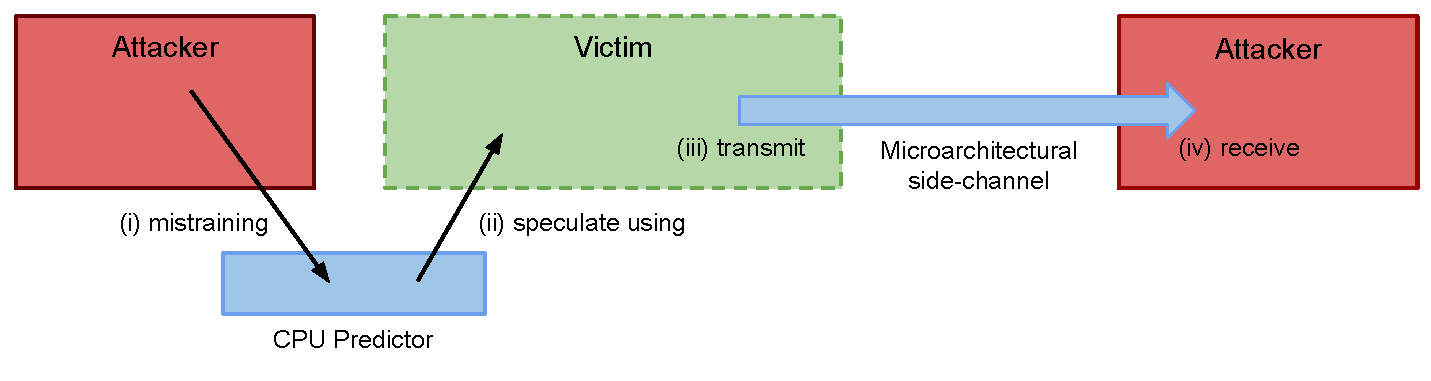
\includegraphics[width=\columnwidth]{AttackSteps.pdf}
    \caption{Steps involved in a transient execution attack.}
    \label{fig:attack-steps}
\end{figure*}

In Spectre V1 for instance, the attacker (i) poisons the branch predictor, (ii) which causes an out of bounds load to pull the victim secret into a register, (iii) so a second memory operation pulls in a cache line whose index is determined by the secret, (iv) so that the attacker can recover the secret by probing which entries are present in the cache.
Exactly how each step is conducted varies between attacks.
For instance, there are many prediction structures within a modern CPU that can be leveraged to reroute speculative control flow, and the access in (ii) can be performed via a gadget in the victim application or entirely using instructions located within the attacker application.
The final receive step is typically noisy and requires some degree of decoding of the observed value to recover the original secret.

Transient execution attacks are possible in settings with code running for two mutually-distrusting entities on the same CPU.
This can be a user application attacking the OS, a user application targeting other user applications, a guest OS exploiting the hypervisor, and so forth.

% \section{Mitigation Approaches}

% There are two main approaches to preventing these attacks: either by modifying software, or altering the CPU design.

% \noindent\textbf{Software:}
% As the embargo period wound down on the original Meltdown and Spectre attacks, operating system vendors and processor makers hurriedly rolled out patches to mitigate these vulnerabilities.
% The patches came at a significant performance cost. 

% These fixes took two forms.
% Hardware vendors released microcode patches for existing processors which modified behavior and added some new functionality to control speculative execution~\cite{intel:l1tf}.
% Meanwhile, operating system makers and other software vendors deployed new versions which blocked the attacks via a combination of software only techniques~\cite{intel:retpoline, linux:kpti} and leveraging the functionality added by microcode~\cite{intel:l1tf}.

% \noindent\textbf{Hardware:}
% Software and microcode approaches to preventing transient execution attacks are severely constrained compared to what is possible by modifying CPU designs themselves.
% For some attacks, straightforward architectural changes completely eliminate the vulnerability with almost no performance overhead and are already deployed in commercially available CPUs.
% For other attacks, performant hardware mitigations remain an active area of research~\cite{OISA, ConTExT}.

\section{Evolution of Mitigation Cost}
Mitigations for transient execution attacks can introduce significant performance costs as surveys by Phoronix have demonstrated~\cite{phoronix:perf-zombieload, phoronix:two-years, phoronix:three-years}.
%For instance, the patches to mitigate Meltdown cause system calls to be up to 8$\times$ slower, while flushing microarchitural buffers to avoid MDS can add thousands of cycles to every context switch.
One goal of this thesis is to gain a more detailed understanding compared to prior work, including by measuring how specific mitigations impact performance.

We start with end-to-end benchmarks to identify which mitigations are relevant to performance.
In selecting workloads, we direct our attention primarily towards security boundaries.
This is because transient execution attacks in one way or another involve leaking information across a boundary and most of the mitigations to prevent them involve performing extra work each time execution crosses a boundary. 
Each selected workload stresses a different boundary: we use LEBench~\cite{ren:lebench} to measure the OS boundary, Octane 2~\cite{google:octane2} to profile JavaScript sandbox overhead, run a few virtual machine benchmarks, and verify that there isn't significant overhead for a few CPU intensive workloads running entirely within a single process.

By varying which mitigations are enabled during each experiment run, we're able to attribute overheads back to the specific mitigations that cause them.
Our test systems vary on many dimensions unrelated to transient execution attacks (like core count, clock speed, and cache size) so our direct comparisons focus on relative differences between configurations of the same system.

On workloads that stress the Linux kernel interface (which have received the most attention) we find there have been substantial improvements with overhead on LEBench going from over 30\% to less than 3\%, and all measured overhead now attributable to a single attack.
By contrast, the performance of JavaScript applications running inside Firefox are impacted by an almost entirely different set of mitigations, which on Octane 2 has caused overhead to remain roughly flat at 20\%.

We aim to understand why some mitigation costs have declined while others have not, and to understand whether moving mitigations from software to hardware truly makes them faster.
Therefore, we also conduct a detailed breakdown of individual mitigation code sequences to investigate their precise cycle costs.
For each mitigation identified by the end-to-end benchmarks, we attempt to measure execution time of the associated instruction or instruction sequence on each of our impacted systems.
Our experiments show some variations between processors in how long individual mitigations take, but demonstrate that the main source of improvement is that some costly mitigations are completed avoided on newer CPUs. 
%The outcome of this investigation explains why overheads to prevent transient execution attacks have significantly declined for some workloads: the overhead of the different software mitigations haven't changed much but the improvements are explained by hardware changes that removed the need for a few of the most expensive mitigations.

\section{Ward}
Mitigations are important for OS kernels because they make a particularly good target for transient execution attacks.
First, an adversary can cause the kernel to speculatively execute code that
leads to leakage of sensitive data. Even though the adversary cannot
inject their own code to execute in the kernel, they can often
have significant influence on what existing kernel code gets executed in
speculative execution, by specifying particular system call arguments or
setting up micro-architectural CPU state such as the branch predictor.
Secondly, an OS kernel has access to all of the state
on the computer. This means that an adversary running in one process
can trick the kernel into leaking state from any other process on the
same computer.

When running on processors designed prior to 2018, the only way for operating systems to prevent transient execution attacks is to use expensive software mitigations.
Such processors will remain in use for years to come and cannot simply be ignored.
%\sys is an operating system architecture designed for such processors.
%It achieves similar security guarantees to traditional OSes equiped with software mitigations but incurs substantially lower overhead.
\sys is a novel operating system architecture that is resilient to transient execution attacks, yet avoids much of the overhead caused by software mitigations when running on these processors.
It is based on the Unmapped Speculation Contract, which describes limits on a processor's speculative behavior: namely that physical memory not mapped into a current or previous page table cannot impact microarchitectural state.

%In \sys, the operating system kernel is divided into multiple domains.
\sys leverages the \contract by dividing the kernel into multiple domains.
The K domain includes all information accessible to the operation system, while each process has its own associated Q domain consisting only of the userspace memory and kernel space data structures related to that one process.
At any given point in time the processor is either executing in userspace, in a Q domain, or in the K domain. 

Notably when executing in a Q domain, \sys is able to avoid many of the expensive software mitigations that would ordinarily be required.
And since \sys is able to handle many system calls and traps entirely in the Q domain, it can achieve considerably better performance on many workloads compared to conventional operating system designs.

\section{Contributions}

One primary contribution of this thesis is to draw attention to the performance critical areas for improving transient execution mitigations, driven by 
(1) a survey mapping end-to-end overheads to the specific mitigations that cause them, and 
(2) detailed microbenchmarking of individual mitigations.
To analyze hardware mitigations for Spectre V2, this thesis also contributes a new technique to measure speculation using ideas from Bölük~\cite{speculating-x86}.

Another contribution is articulating the Unmapped Speculation Contract, which describes upper limits of what speculative execution attacks can and cannot do.
This thesis then demonstrates the benefits of the contract
by presenting \sys{}, a novel kernel architecture that uses
selective kernel memory mapping to avoid some of the costly transient execution
mitigations required on older Intel processors.

\section{Outline}
The following chapter presents an end-to-end performance evaluation and goes into detail on each major attack describing both background on how it works as well as analyzing its impact on each evaluated system (\autoref{ch:evolution}).
We then proceed to introduce the Unmapped Speculation Contract, which encapsulates some security guarantees that we believe even old processors are able to provide, and describe the \sys kernel design which improves the performance of OS intensive workloads by leveraging it (\autoref{ch:ward}).
Afterwards is an overview of related work (\autoref{s:related}).
We follow up with some discussion and ideas for future work (\autoref{s:discussion}), and then conclude (\autoref{s:concl}).
